\chapter{相关工作}

本章将首先介绍面诊技术的概念和发展,然后介绍当前比较流行的基于面诊技术的应用。
\subsection{面诊技术}

\section{面诊技术的应用}

\begin{figure}[h]
    \centering
    \subfigure[面诊仪]{
        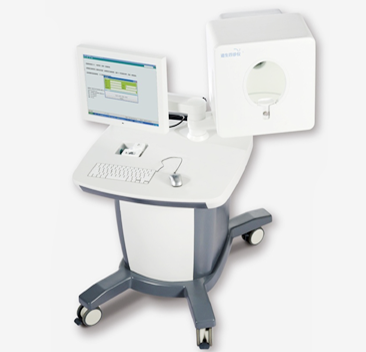
\includegraphics[height=6cm]{images/mzy.png}
    }
    \subfigure[云中医智能镜]{
        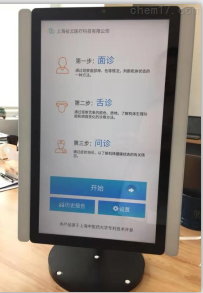
\includegraphics[height=6cm]{images/yzy.png}
    }
    \caption{面诊技术的应用}
    \label{fig:med}
\end{figure}

\subsection{面诊仪}
面诊仪如道生面诊仪\cite{邸丹2016手持式舌象仪的研制}是目前某些医院用来采集面部信息的设备,需要在中医医师的指导下,进行舌相面色诊断信息采集,供中医医师进行判断; 


\subsection{云中医}

\begin{figure}[h]
    \centering
    \subfigure[主界面]{
        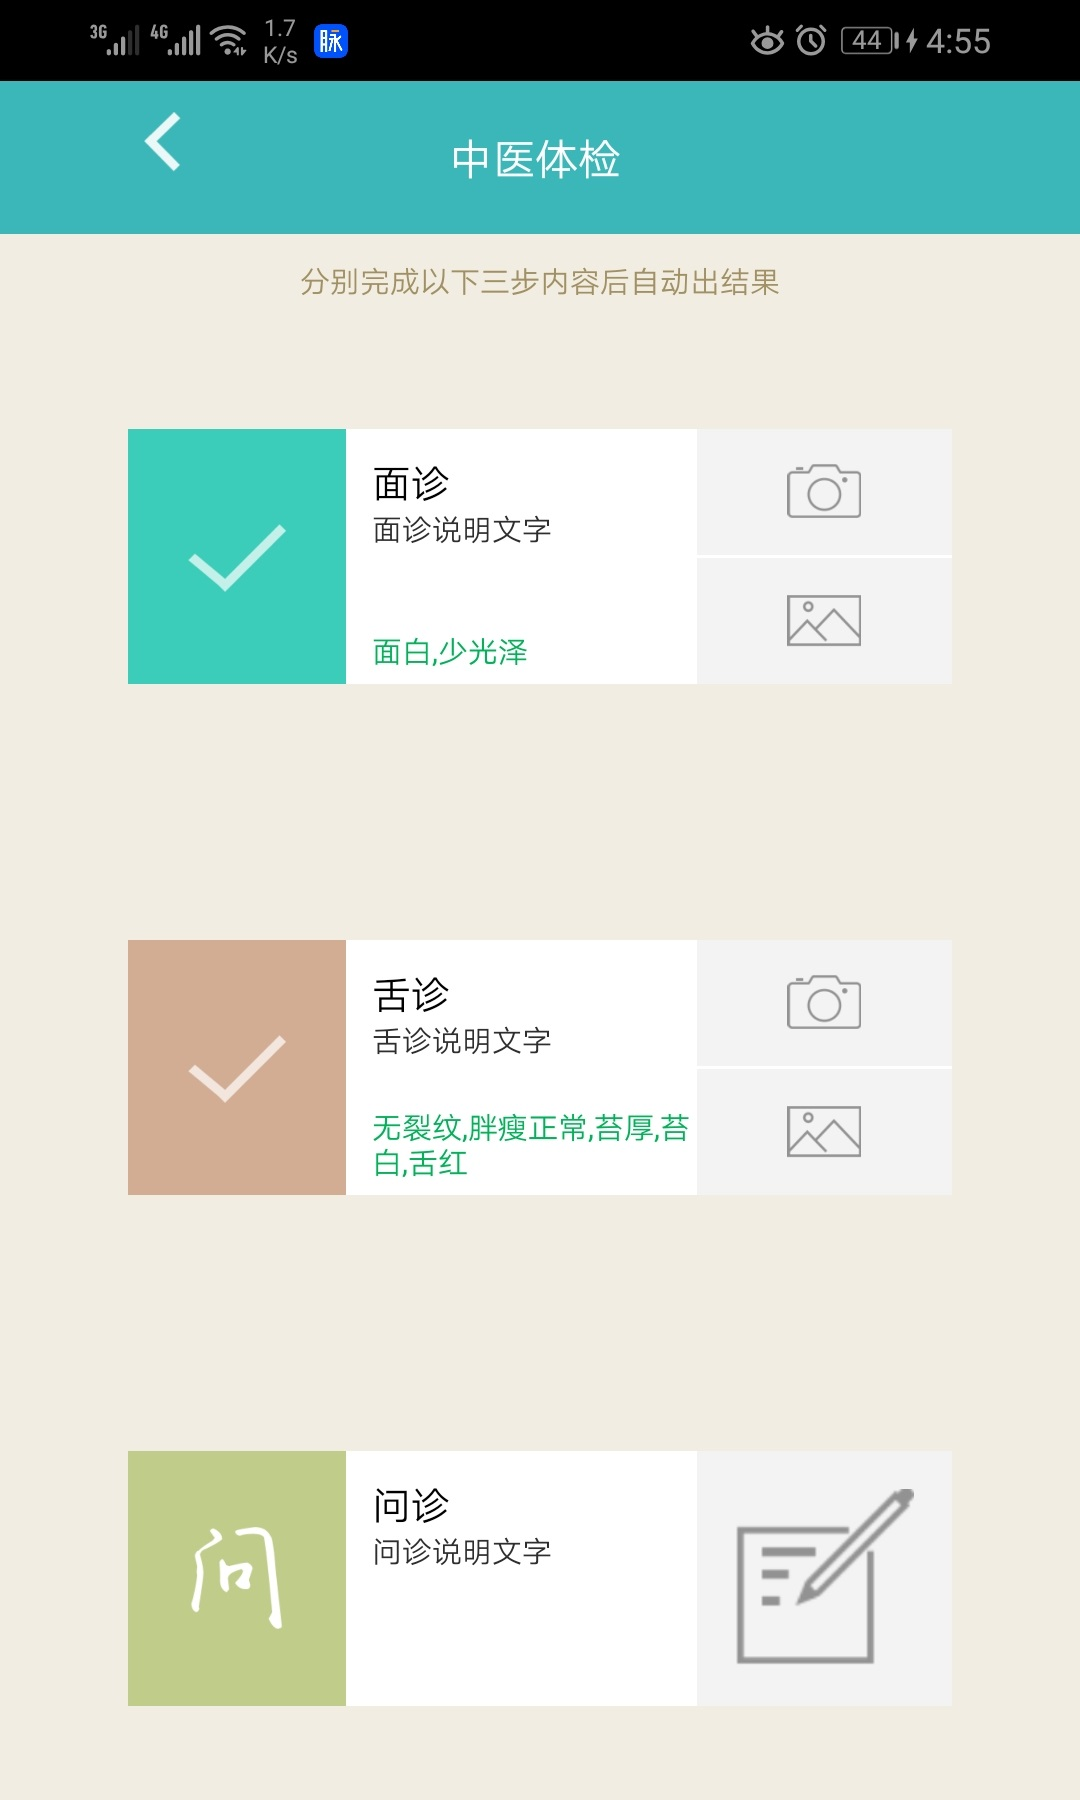
\includegraphics[width=4.5cm]{images/main1.jpg}
    }
    \subfigure[问诊]{
        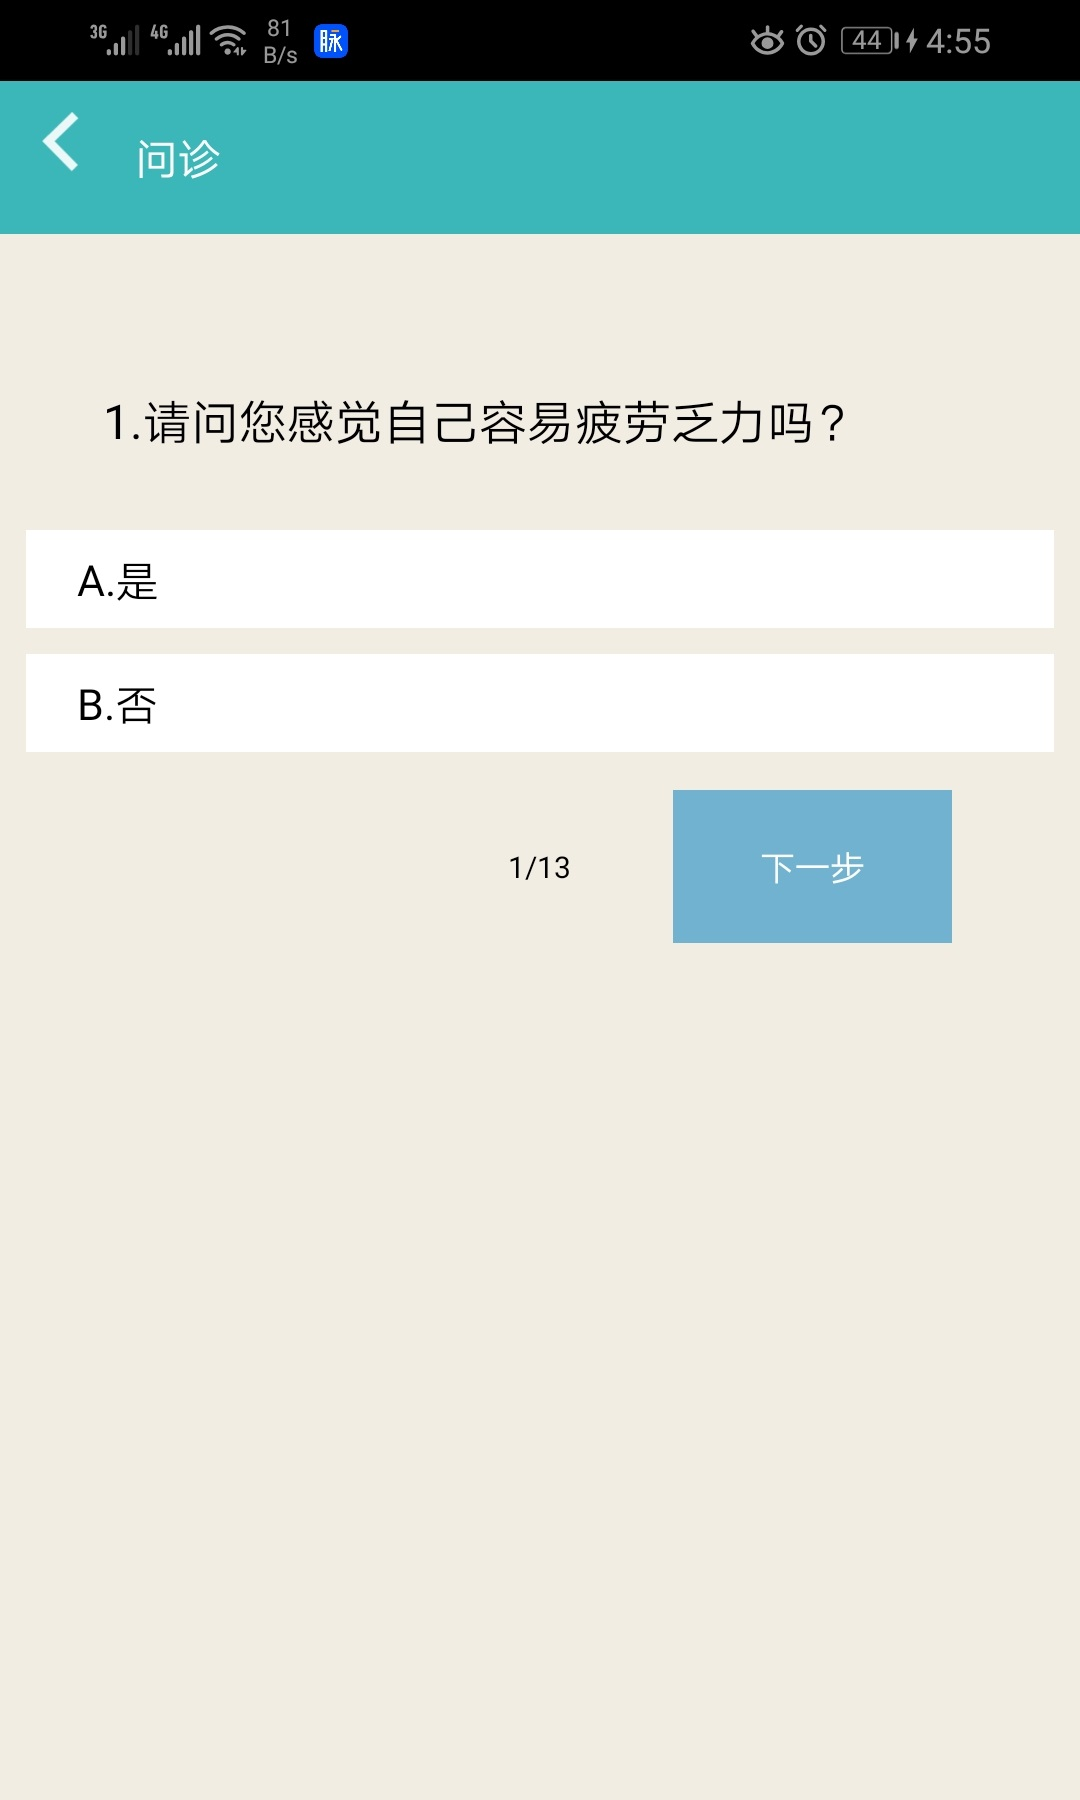
\includegraphics[width=4.5cm]{images/main2.jpg}
    }
    \subfigure[健康报告]{
        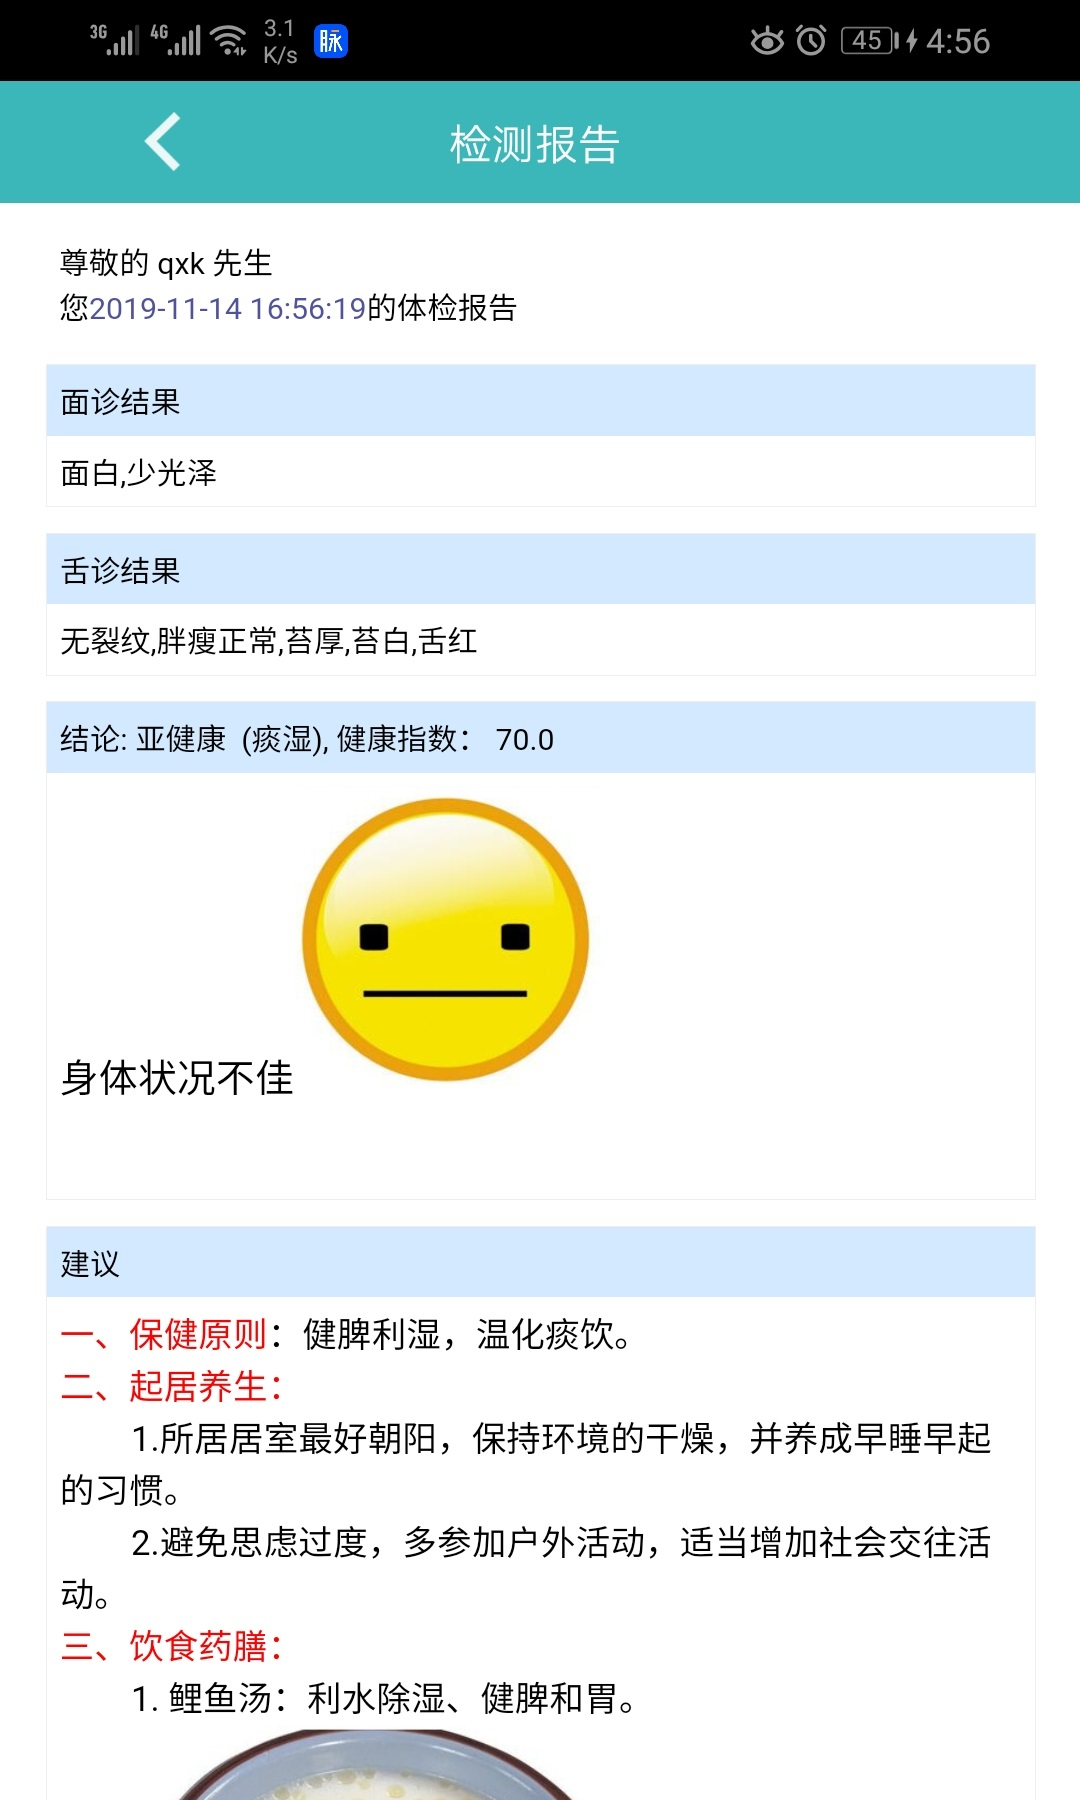
\includegraphics[width=4.5cm]{images/main3.jpg}
    }
    \caption{技术探针}
    \label{fig:main}
\end{figure}
云中医是复旦大学计算机学院张文强老师和上海中医药大学合作开发的一款面诊应用,旨在为用户提供一个方便的自我诊断和健康管理平台,目前主要应用场景是各大社区、诊所以及健康辅助机器人。该应用以中医面诊、舌诊、问诊理论为指导,在手机上模拟实现了诊断的过程:
用户需要依次对自己的面部和舌头进行拍照,回答一些与自己健康状况相关的问题,最终会收到一份完整的健康报告和一些健康建议。

云中医app的主要界面及使用流程如图 \ref{fig:main}所示:用户进入诊断页面之后,会看到三个区域:面诊、舌诊、问诊。面诊和舌诊通过拍照或者上传图片完成,问诊是通过依次回答13个问题来完成。
依次完成面诊、舌诊、问诊后,系统会给出用户的体质和健康分数,并且给出对应的健康建议。

云中医虽然功能比较齐全,但是其主要应用场景是社区和诊所等公共环境,其中包括云中医诊断机器人\footnote{http://www.sohu.com/a/135358060\_205169/},云中医智能镜\cite{李雪2016},云中医应用\cite{钱鹏基于云中医的健康监测方法及系统}等,缺乏日常健康环境下的用户研究和交互研究。


\section{人机交互研究与设计方法}
\cite{lazar2017research}
% 定性研究, 强调context的重要性,以人为中心,重视用户的体验。
人机交互(Human-Computer Interaction)的研究以人为中心,涵盖计算机科学、社会学、心理学等学科,重视技术如何更好地为人服务。
% 研究方法

% 数据采集方法

% 技术探针, 文化探针 等

\section{本章小结}
本章主要介绍了日常健康交互技术和读脸技术的相关工作。
第一部分介绍了读脸技术的广泛应用。随着技术的发展,读脸技术的应用非常广泛。从安防和访问控制,到情绪识别,读脸技术也广泛用于医疗领域识别病人信息,远程监测患者, 甚至用于检测健康状态。
但是本文关注的医疗领域的读脸技术的应用,不管是各种管理系统还是对应的硬件设备,大多是为专业医护人员设计的,面诊技术关于日常健康场景下的面诊技术如何设计还需要进一步的探索。
第二部分介绍了人机交互领域在日常健康方面的研究,从传统的慢性疾病管理到支持用户更健康生活方式的研究,同时指出当前的日常健康的研究,还未探索面部信息作为健康指标的技术。

